%%=============================================================================
%% POC Outsystems
%%=============================================================================

\chapter{POC: Outsystems}
\label{ch:outsystems-poc}

%% TODO: Hoe ben je te werk gegaan? Verdeel je onderzoek in grote fasen, en
%% licht in elke fase toe welke stappen je gevolgd hebt. Verantwoord waarom je
%% op deze manier te werk gegaan bent. Je moet kunnen aantonen dat je de best
%% mogelijke manier toegepast hebt om een antwoord te vinden op de
%% onderzoeksvraag.

% TODO: kleine inleiding

\section{Voorbereiding}

\subsection{Van 0 tot de eerste app uitvoering}

De eerste stap is om een account aan te maken, hierna kan de Outsystems software geïnstalleerd worden (Service Studio als gewone IDE en Extension Studio om uitbreidingen te maken).\\
In de persoonlijke omgeving kan naast het maken van een nieuwe app community componenten van de Forge ook rechtstreeks geïnstalleerd worden. \\
Bij het maken van een app zijn er vijf keuzes: reactive of traditionele web app, tablet of telefoon app en ten laatste ook een service. Er is voor reactive gekozen omdat er in de POC in PowerApps twee versies gemaakt zijn en de app dus op meerdere platformen moet kunnen gebruikt worden. Na de creatie van de app wordt ook een module aangemaakt.\\
De eenvoudigste manier om data te introduceren is door een Excel file op te laden. De data hieruit wordt naar een cloud instantie van SQL Server opgeslagen.\\
Als de app gestart wordt moeten Outsystems credentials opgegeven worden.

Dit is de basis om de requirements uit te kunnen beginnen werken maar eerst nog wat uitleg bij het gebruik van de IDE.

\subsection{IDE en begrippen}
Er zijn een aantal functies aanwezig, hier uitgelegd per mogelijk weergavepaneel (Zie Figuur~\ref{fig:ide-overzicht}):
\begin{itemize}
    \item \textbf{Centraal:} Hier kunnen de UI flows (onderlinge verhouding van de schermen), ontwerpweergave van een scherm of een actie/methode weergave staan.
    \item \textbf{Links:} Een overzicht van de beschikbare UI controls of actie stappen.
    \item \textbf{Rechts:} Context views voor de processen, interface, de logica en de data. Aangevuld met een properties paneel wanneer toepasselijk.
\end{itemize}

\begin{figure}[h!]
     \makebox[\textwidth]{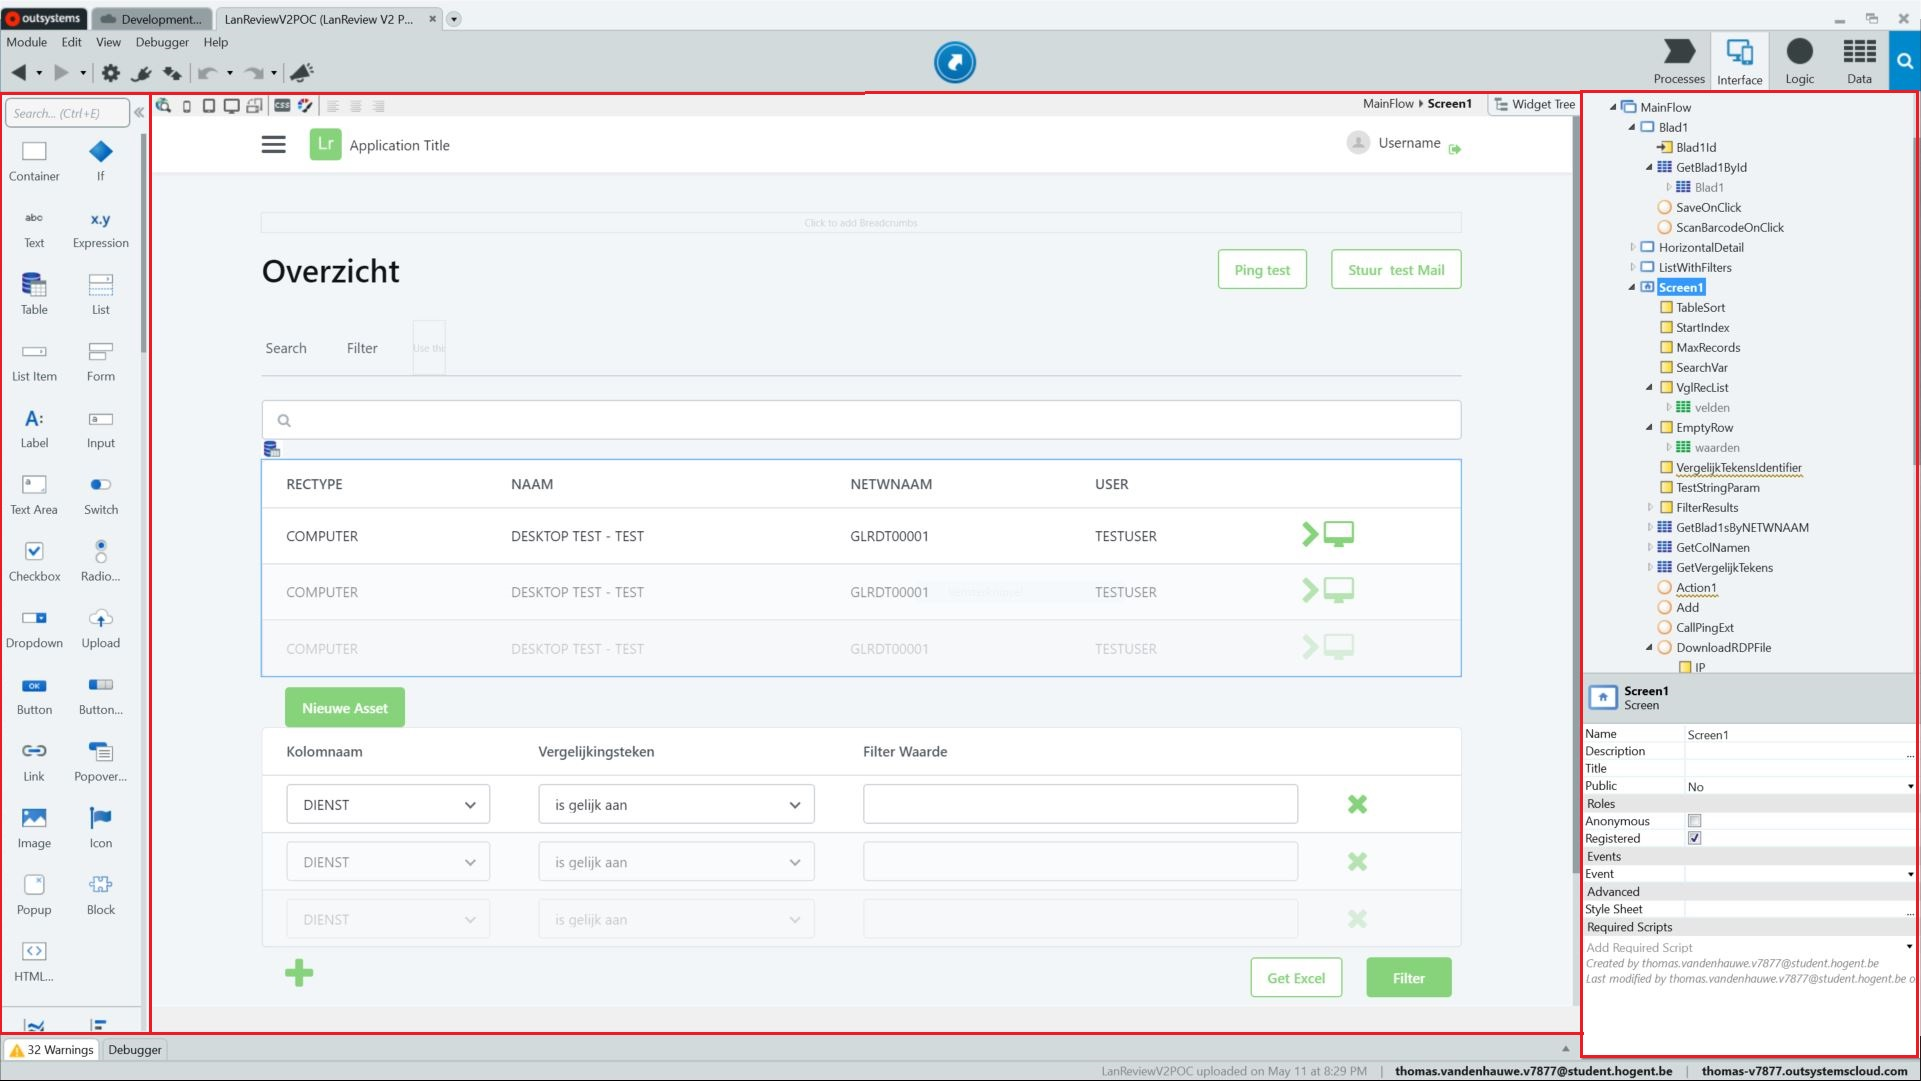
\includegraphics[width=1.3\linewidth]{ide-overzicht-edited.JPG}}
     \caption{Overzicht van de Outsystems Service Studio.}
     \label{fig:ide-overzicht}
\end{figure}

Er zijn een aantal begrippen die gekend moeten zijn bij het maken van applicaties.
\begin{itemize}
    \item TrueChange Debugger:\\
    Zoals verwacht van een debugger kunnen breakpoints gezet worden en zijn tijdens uitvoering de waarden van de actieve variabelen in te kijken. Het interessante is dat hiernaast de app geanalyseerd wordt en performantie en security aanbevelingen teruggegeven worden.
    \item One Click Publish:\\
    Stappen uit traditionele software ontwikkeling om een app beschikbaar te stellen (verifiëren, compileren, uploaden en publiceren van code) worden geautomatiseerd met één knop. Als de verificatie faalt moeten de fouten eerst uit de app gehaald worden.
    Dit betekent ook dat wijzigingen altijd online worden gezet voor het resultaat bekeken kan worden.
    \item AI Assisted development:\\
    Tijdens ontwikkeling wordt AI gebruikt om onder andere sleutelwoorden en app context te analyseren en op basis hiervan acties aan te bevelen. Een voorbeeld van het gebruik ervan in de POC was dat wanneer een actie aangemaakt werd in de lijst op het hoofdscherm er voorspeld werd dat er een detailweergave nodig was. Dit detailscherm en bijbehorend formulier werd automatisch gegenereerd.
    \item Aggregate VS SQL Query:\\
    Er zijn twee manieren om data te queryen. Een aggregate is eenvoudig te declareren en beter geoptimaliseerd in Outsystems dan een gewone SQL query. Die is echter flexibeler en het gebruik ervan wordt aangeraden wanneer iets niet mogelijk is met een aggregate. Beiden werden gebruikt in de POC en komen verder aan bod.
    %\item Datatypen:
    %\item Expressie taal:
    %\item REST acties:
    %\item Meer over de Extenstion Studio:
\end{itemize}

\section{Model van Opstelling}

\begin{figure}[h!]
    \centering
    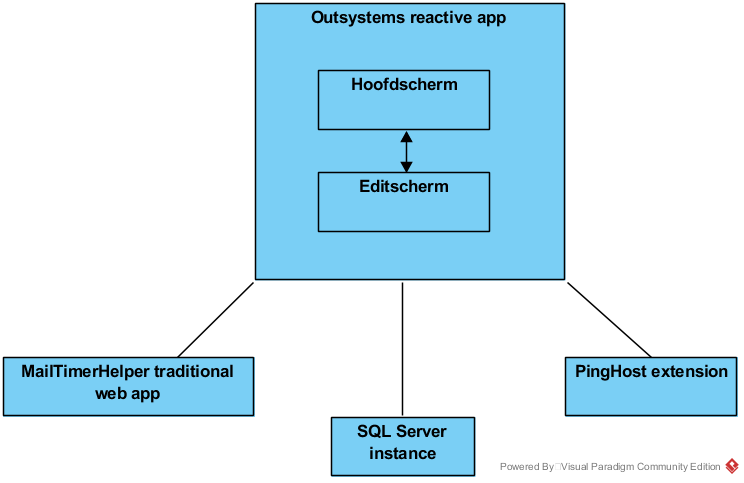
\includegraphics[width=0.8\linewidth]{Outsystems-POC-model.png}
    \caption{Model van de Outsystems proof-of-concept.}
    \label{fig:Outsystems-POC-model}
\end{figure}

\section{Requirements}

\subsection{Must have}

\subsubsection{Prijs}
\label{subsec:os-prijs}

De Personal Environment\footnote{What's an OutSystems personal environment? - \url{https://success.outsystems.com/Support/Personal_Environment/What's_an_OutSystems_personal_environment}} (gratis versie) legt geen beperkingen op de bruikbare functionaliteit of hoe lang deze omgeving beschikbaar is. Dit betekent echter niet dat er geen limieten zijn. De hamvraag is of deze limieten aanvaardbaar zijn voor het gebruiksscenario van de POC. Ze worden daarom één per één afgetoetst:

\begin{itemize}
    \item Maar één ontwikkelaar in de omgeving, er is geen samenwerking mogelijk.\\
    $\rightarrow$ De app is niet zodanig complex dat meerdere personen nodig zijn om te ondersteunden of verder uit te bouwen.
    \item Database capacitiet is gelimiteerd tot 2GB.\\
    $\rightarrow$ De bij te houden informatie over de meer dan 1000 assets valt hier nog steeds ruim onder.
    \item Indien de app een maand niet gebruikt wordt gaat de omgeving 'in slaap' en moet de app opnieuw gegenereerd worden voor deze opnieuw gebruikt kan worden.\\
    $\rightarrow$ De app zal dagelijks gebruikt worden dus dit zal nooit een risico worden.
    \item Cloud resources worden gedeeld met andere gebruikers, er is geen service garantie.\\
    $\rightarrow$ De app eist geen intens resource gebruik. 
    \item Er is geen harde limiet op het aantal toegestane app gebruikers maar als de vorige items in beschouwing genomen worden zal een app bruikbaar zijn tot maximum 100 personen.\\
    $\rightarrow$ Maximum zes personen zullen de app gebruiken.
\end{itemize}

De marktleidende low-code platformen gefocust op professionele ontwikkelaars zijn duurder dan de concurrentie. Mendix en Outsystems rekenen meer dan \euro2000 voor hun basisplan (Zie Tabel \ref{tab:price-outsystems} en \ref{tab:price-mendix}). Het was daarom belangrijk dat de POC binnen de limieten bleef, de meerprijs zou niet worden aanvaard.

\subsubsection{Overzicht kunnen geven van belangrijkste info voor elk toestel in het netwerk}

Dit wordt gedaan via een hoofdscherm met een overzicht van de assets en een detail/editscherm dat meer informatie toont (Zie Figuur \ref{fig:os-hoofd} en \ref{fig:os-detail}).
Waar dit bij PowerApps gegenereerd kan worden uit data kunnen dezelfde resultaten eenvoudig bekomen worden met behulp van AI geassisteerde acties.
\begin{enumerate}
    \item Een nieuw scherm aanmaken en kiezen voor een lijstweergave sjabloon.
    \item De data slepen naar het tabel element volstaat na wat kolomaanpassingen om een gewenste weergave van de data te krijgen. Achter de schermen wordt een aggregate aangemaakt die de rijen ophaalt uit de databank.
    \item Als een knop aangemaakt wordt in de rij zal als actie aanbevolen worden dat er een nieuw scherm wordt aangemaakt met een detailweergave. In de achtergrond wordt de id van het rij item meegegeven om in het detailscherm een aggregate in te stellen die deze id gebruikt om alle data van het item op te halen en te tonen.
    \item In het detailscherm kan de layout aangepast worden naar wens en kan validatie ingesteld worden.
\end{enumerate}

\begin{figure}[h!]
    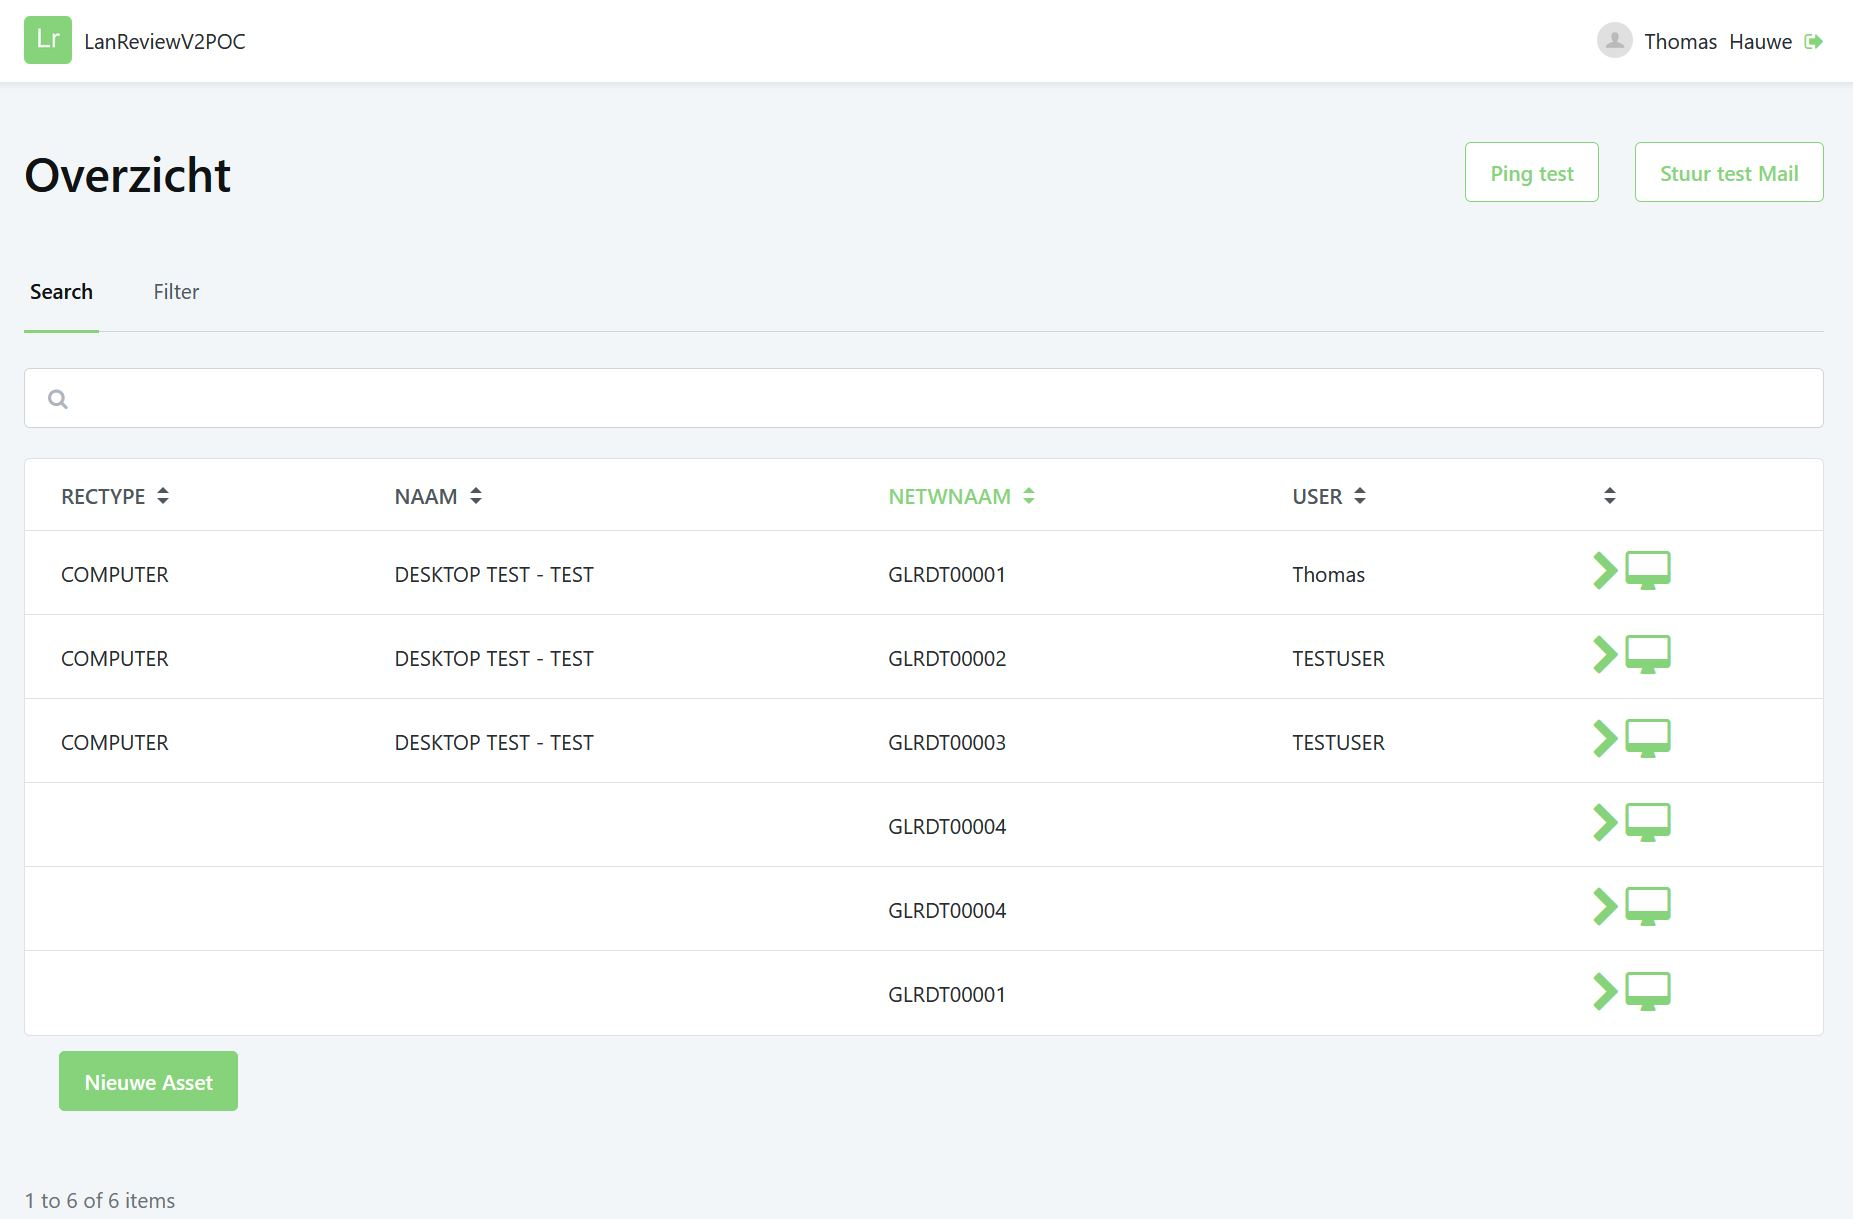
\includegraphics[width=\linewidth]{os-hoofd.JPG}
    \caption{Hoofdscherm Outsystems POC}
    \label{fig:os-hoofd}
\end{figure}

\begin{figure}[h!]
    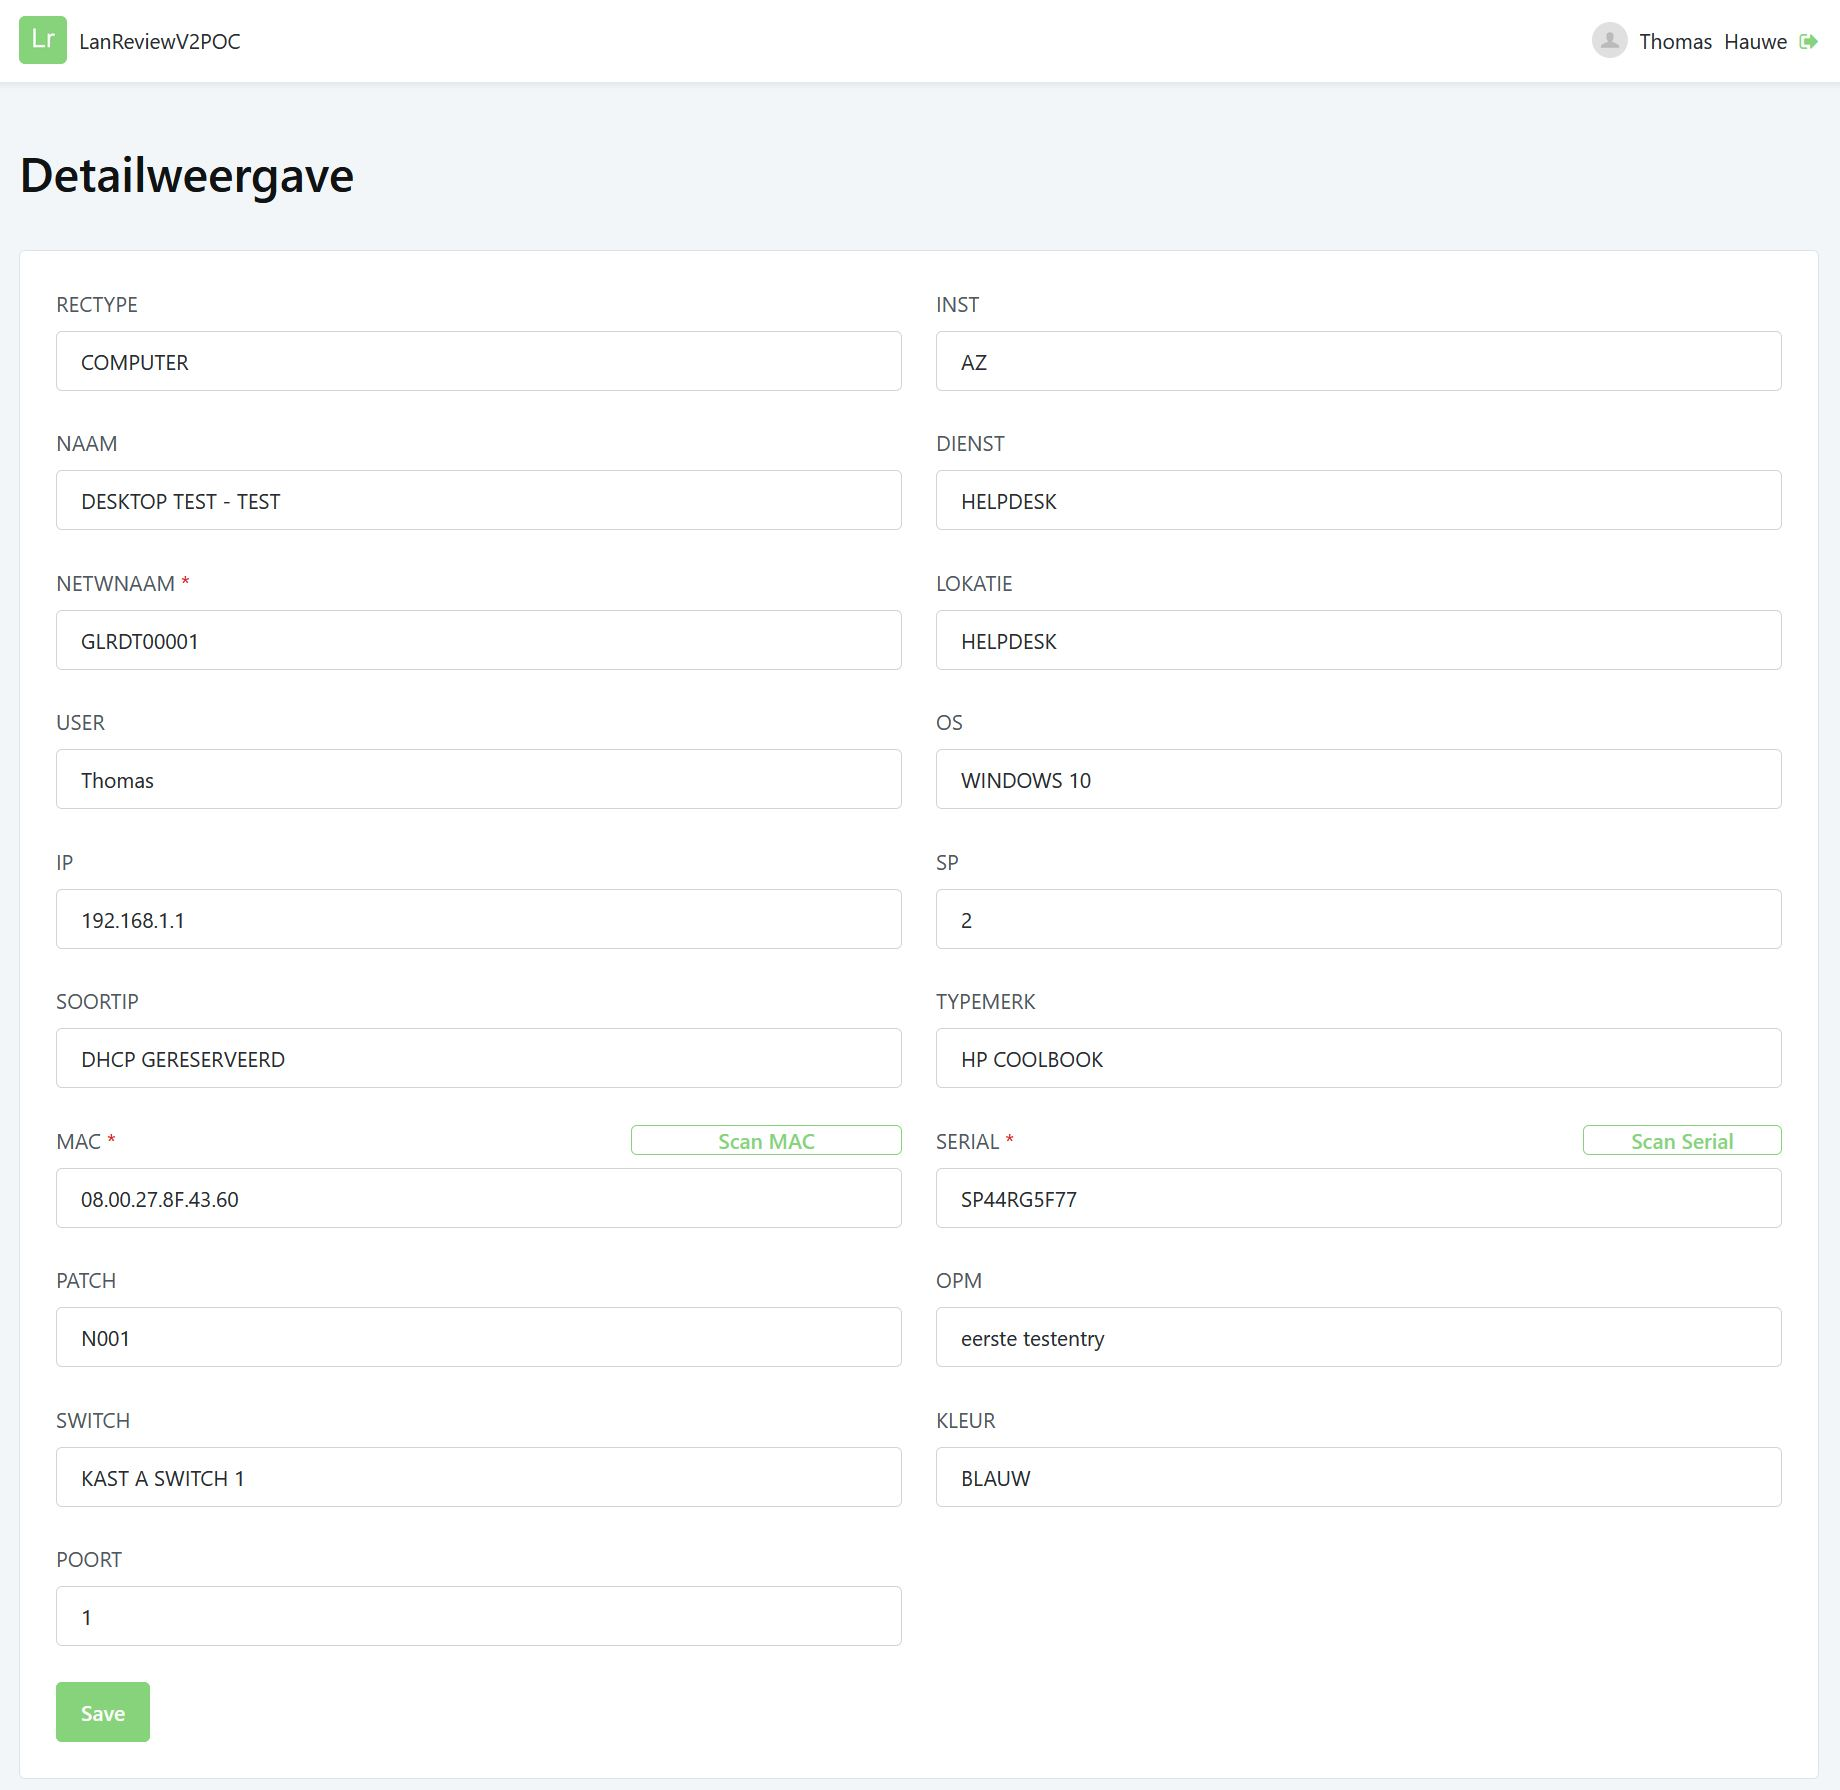
\includegraphics[width=\linewidth]{os-detail.JPG}
    \caption{Detailscherm Outsystems POC}
    \label{fig:os-detail}
\end{figure}

Dit instellen van validatie is belangrijk. Omdat de data recent werd geïmporteerd naar de SQL instantie zijn er geen specifieke regels op ingesteld. Als een externe databron gebruikt werd (bijvoorbeeld SharePoint) had dit wel het geval kunnen zijn.\\
Outsystems heeft automatische client side validatie. \autocite{OutSystemsDocs} In de formulier widget heeft elk inputveld geassocieerd met een kolom een nodig inputtype (zoals mail, datum, tekst) toegewezen gekregen, elke input is standaard ook verplicht (via het 'mandatory' property). Het formulier zelf heeft een Valid boolean property dat op false wordt gezet als validatie in één van de inputs zou falen. Controle hierop gebeurt in de client actie gekoppeld aan de knop om toe te voegen of te wijzigen. Het is deze actie die gewijzigd moet worden volgens het specifieke scenario. (Zie Figuur~\ref{fig:os-validatie-tesamen})

Gaat het om het toevoegen van een nieuwe entry of wijzigen van een bestaande? Indien het een nieuwe is wordt gekeken of het ingevulde Netwnaam uniek is via de server actie 'NetwNaamUnique'. Deze zal een aggregate uitvoeren waarin een filter toegepast is  die kijkt of de meegegeven Netwnaam matcht aan een waarde uit de NETWNAAM kolom. Indien de netwerknaam uniek is wordt verdergegaan met de formuliervalidatie. Indien niet wordt een error message gekoppeld aan de textinput van de Netwnaam en stopt de actie.

\begin{figure}[h!]
    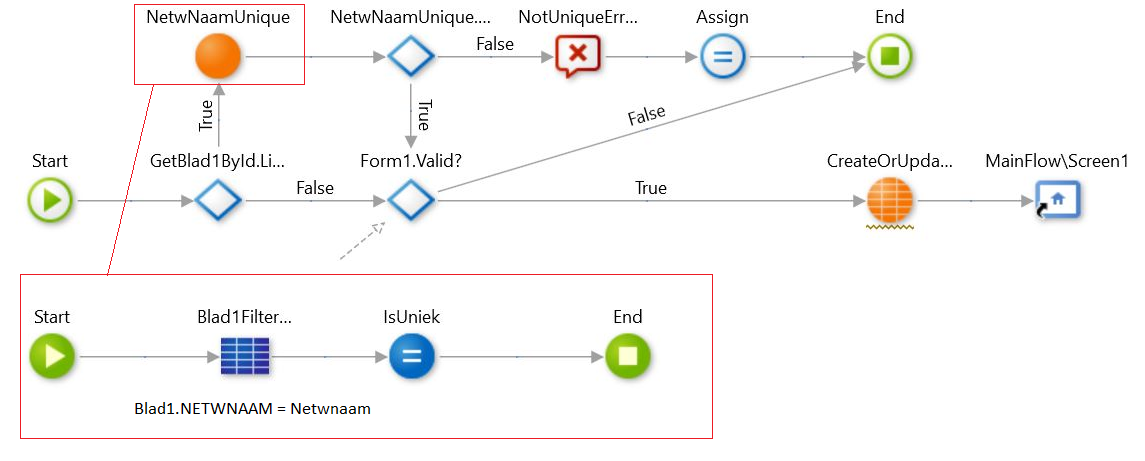
\includegraphics[width=\linewidth]{os-validatie-tesamen.png}
    \caption{Uitbreiding van de standaard formuliervalidatie.}
    \label{fig:os-validatie-tesamen}
\end{figure}

\subsubsection{Filtering / rapportage}

\textit{Filter}

Zoeken en filteren is in tabbladen gescheiden en ook hun resultaten worden in aparte Table controls weergegeven.

$\rightarrow$ Search:

Voorbereidend wordt er een filter ingesteld in de reeds bestaande aggregate (die items ophaalt om weer te geven in het hoofdscherm) die een zoekvariabele zal matchen aan elke kolom.
Er wordt een zoekveld toegevoegd aan het scherm en deze zoekvariabele wordt eraan gekoppeld. Als OnChange event wordt een client actie uitgevoerd die de aggregate ververst (en de filter opnieuw uitvoert met de gewijzigde zoekvariabele).

\begin{lstlisting}
Blad1.NETWNAAM like "%" + SearchVar + "%" or Blad1.RECTYPE like "%" + SearchVar + "%" or ... or Blad1.KLEUR like "%" + SearchVar + "%"
\end{lstlisting}

$\rightarrow$ Filter:
\begin{itemize}
    \item \textbf{Vorm en datatypen:}\\
    De filter bouwen gebeurt via een dynamisch groeiende lijst waarbij elke rij bestaat uit een keuzeveld voor de kolom, de soort vergelijking en de tekst om op te filteren.\\
    Er moeten enkele datatypen voorbereid worden om dit mogelijk te maken:
    \begin{itemize}
        \item Statische entitieit die alle kolomnamen bevat.
        \item Statische entitieit die alle mogelijke vergelijkingen/operators bevat.
        \item Structuur die de filterwaarden van een rij zal vasthouden. Dit is een samengesteld type, het bevat:
        \begin{itemize}
            \item Identifier van de entiteit met kolomnamen.
            \item Identifier van de entiteit met operators.
            \item Een Text variabele met de filterwaarde.
        \end{itemize}
    \end{itemize}
    In de interface moeten nog twee variabelen aangemaakt worden: een Record List van de 'FilterVelden' (zal elke filterwaarde bevatten) en een Record van 'FilterVelden' (stelt een lege rij voor). Ten laatste moet wat hierboven aangemaakt is correct toegewezen worden aan de properties van de dropdowns.(Zie Figuur~\ref{fig:data-en-dropdown})
    Het Advanced Filter Builder\footnote{\url{https://www.outsystems.com/forge/component-overview/365/advanced-filter-builder}} Forge component werd gebruikt om hier wijs uit te geraken.\\
    \item \textbf{Query:}\\
    De 'Filter' knop voert de 'FilterOnClick' client actie uit die op zijn beurt de 'Filter' server actie uitvoert. De Record List wordt als argument meegegeven.\\
    De 'Filter' actie (Zie Figuur \ref{fig:filter-action}):
    \begin{enumerate}
        \item Controleren of de Record List leeg is. Indien ja, stopt de uitvoering.
        \item De eerste entry naar een string converteren. 
\begin{lstlisting}
GetColNamen(VglRecList[0].velden.ColNaamAtt).ColNamen.Naam + " " + GetVergelijkTekens(VglRecList[0].velden.VergelijkTekenAtt).VergelijkTekens.Teken + " '" + VglRecList[0].velden.FilterWaarde + "'"
\end{lstlisting}
        \item Controleren of er meerdere records zijn. Indien ja, wordt er gelooped en wordt de string verder aangevuld via onderstaande expressie:
\begin{lstlisting}
TestStringParam + " and " + GetColNamen(VglRecList.Current.velden.ColNaamAtt).ColNamen.Naam + " " + GetVergelijkTekens(VglRecList.Current.velden.VergelijkTekenAtt).VergelijkTekens.Teken + " '" + VglRecList.Current.velden.FilterWaarde + "'"
\end{lstlisting}
        \item De SQL query uitvoeren. Een opmerking hierbij is dat de 'expand inline' optie actief moet staan om de gebouwde string effectief te kunnen gebruiken als argument. De query zelf is een simpele WHERE met door AND aaneengeschakelde evaluaties. (Figuur~\ref{fig:sql-query})
    \end{enumerate}
    De gereturnde filterresultaten worden in een aparte Table geplaatst. Dit maakt het exporteren als report later makkelijker.\\
    De gevonden beperkingen zijn dat het evalueren met sommige kolommen niet juist werkt en dat de performantie lager is dan bij een aggregate.
\end{itemize}

%[filter-afb]

\begin{figure}[h!]
    \centering
    \begin{subfigure}[b]{0.3\linewidth}
        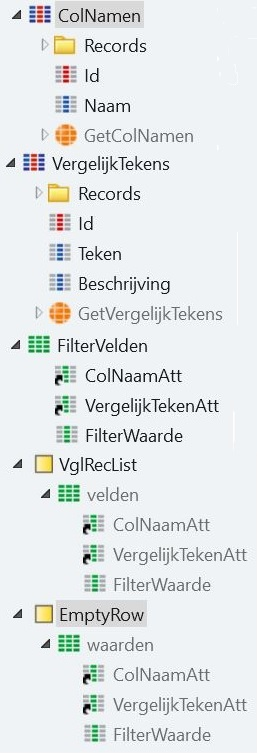
\includegraphics[width=\linewidth]{data-tesamen.jpg}
        \caption{Overzicht van de datastructuren en variabelen.}
    \end{subfigure}
    \begin{subfigure}[b]{0.5\linewidth}
        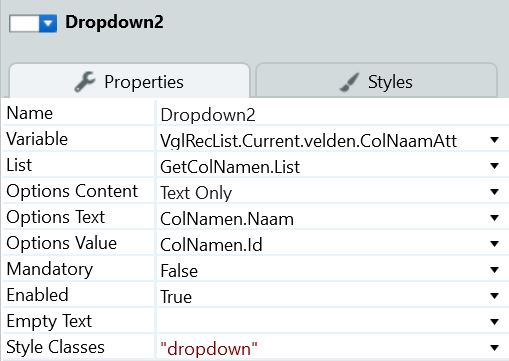
\includegraphics[width=\linewidth]{dropdown-props.JPG}
        \caption{Hoe de data aan de dropdown met kolomnamen gekoppeld wordt.}
    \end{subfigure}
    %\begin{subfigure}[b]{0.5\linewidth}
    %    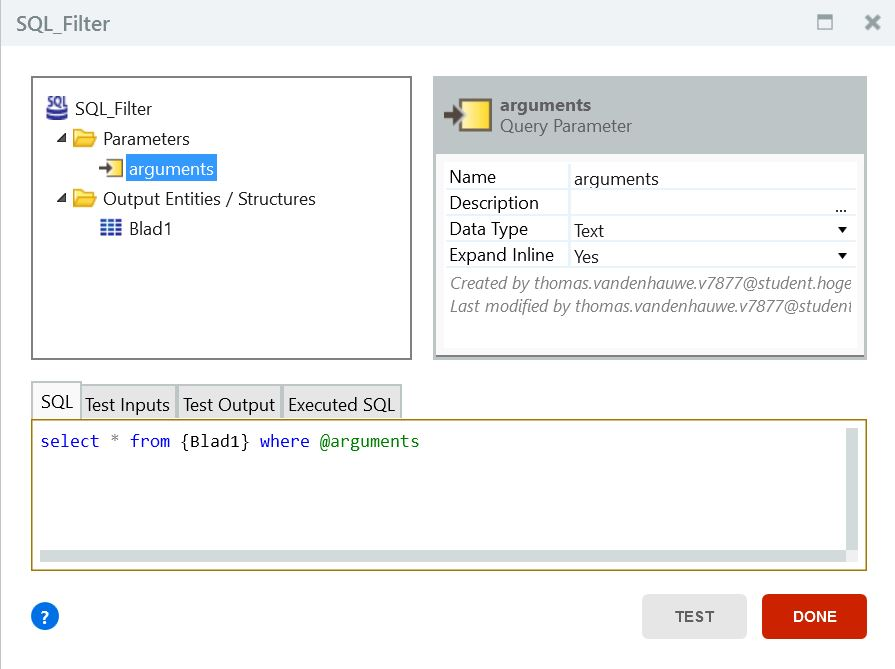
\includegraphics[width=\linewidth]{sql-query.JPG}
    %    \caption{De SQL query.}
    %\end{subfigure}
    \caption{Overzicht van de filtering voorbereidingen.}
    \label{fig:data-en-dropdown}
\end{figure}

\begin{figure}[h!]
    \centering
    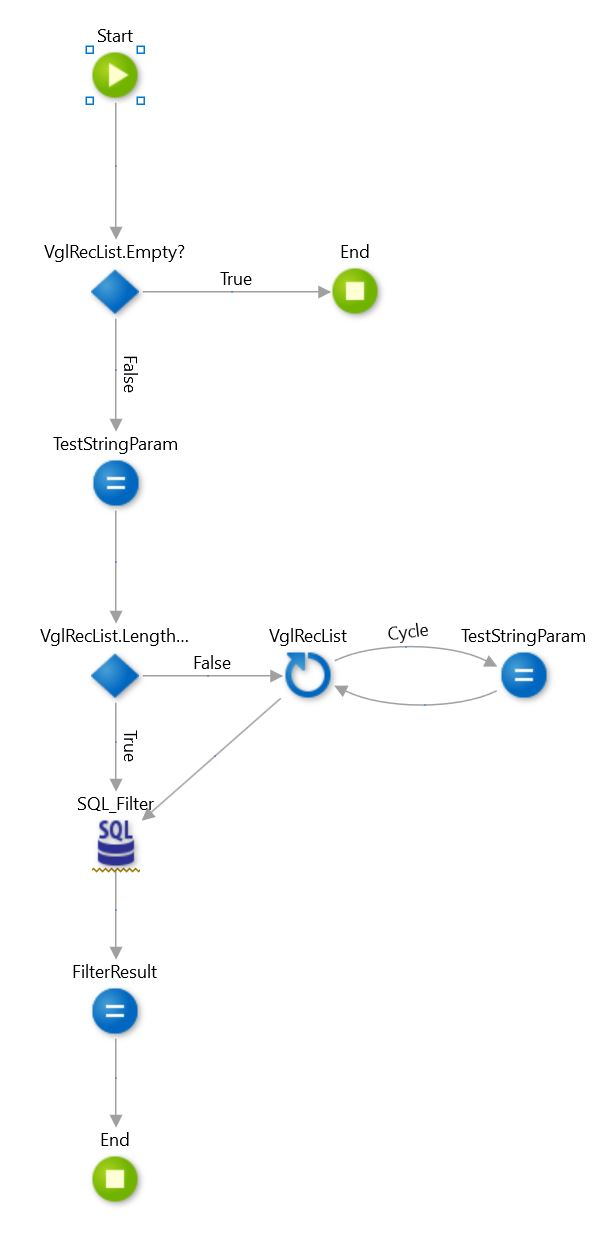
\includegraphics[width=0.5\linewidth]{filter-action.JPG}
    \caption{De Filter actie.}
    \label{fig:filter-action}
\end{figure}

\begin{figure}[h!]
    \centering
    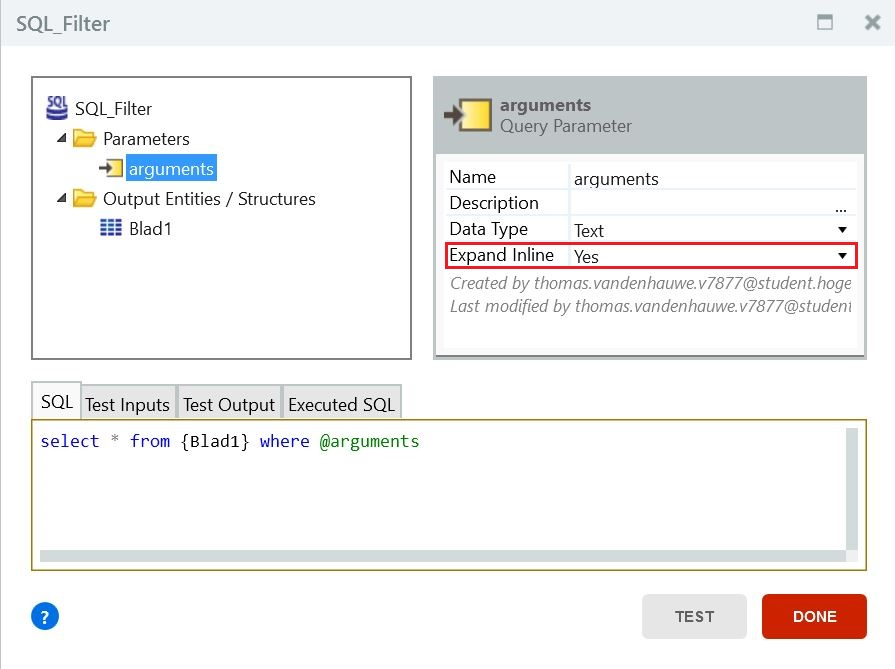
\includegraphics[width=0.75\linewidth]{sql-query-edited.JPG}
    \caption{De SQL query.}
    \label{fig:sql-query}
\end{figure}

\textit{Reporting}

Downloadacties zijn goed ondersteund. Door een download control als eindpunt van een actie te zetten wordt de geconfigureerde inhoud ervan aangeboden in een download prompt. De specifiek geconfigureerde acties om dit te bereiken worden opgeroepen wanneer er een gewenste dataset gefilterd staat en op de 'Get Excel' knop geduwd werd.
\begin{enumerate}
    \item \textbf{GetExcel (Client actie):} Het filterresultaat naar de server actie doorgeven en de gereturnde Excel file te downloaden zetten.
    \item \textbf{PrepareExcel (Server actie):} De filterresultaten converteren naar een Excel bestand via de 'Record List to Excel' stap.
\end{enumerate}

%[afb van prompt om tedownloaden] ?

\begin{figure}[h!]
    \centering
    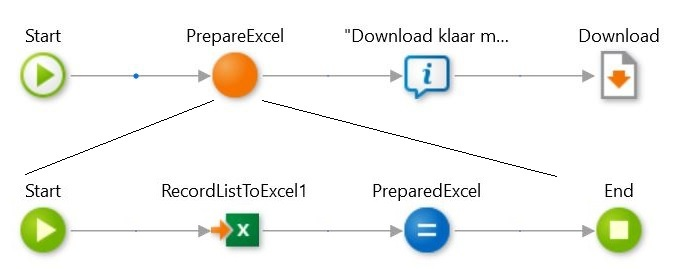
\includegraphics[width=0.8\linewidth]{report-tesamen.jpg}
    \caption{De client en server actie om een rapport te downloaden.}
    \label{fig:report-tesamen}
\end{figure}

\subsubsection{RDP / Ping}

\textit{RDP (Remote Desktop Protocol)}

Omdat de POC in de cloud draait is deze functionaliteit niet direct op te roepen, mogelijke workarounds:
\begin{itemize}
    \item \textbf{Workaround 1:} Client side javascript, specifiek een ActiveX plugin gebruiken om shell commando's uit te voeren\footnote{How to Run cmd.exe with parameters from javascript - \url{https://stackoverflow.com/questions/10186813/how-to-run-cmd-exe-with-parameters-from-javascript}}.\\
    $\rightarrow$ 'ActiveX not defined' error. Dit is enkel mogelijk met oudere versies van Internet Explorer. Het is ook logisch dat dit niet meer ondersteund is vanuit security aspect.
    \item \textbf{Workaround 2:} Een 'link' control en de href property laten wijzen naar een lokale RDP file.\\
    $\rightarrow$ Niet flexibel genoeg: de rdp config file zou elke keer aangepast moeten worden met het relevante IP-adres.
    \item \textbf{Workaround 3:} De webbrowser waar de POC in werkt configureren om custom urls te kunnen gebruiken (zoals rdp://). Vanuit de app naar dat soort url navigeren via de ingebouwde 'RedirectToUrl' functie.\\
    $\rightarrow$ Te veel extra configuratie buiten Outsystems en twijfelachtige ondersteuning.
    \item \textbf{Workaround 4:} Een RPD file maken voor de gewenste pc en downloaden/uitvoeren. Dit past delen toe zoals gezien in het RDP File Creator\footnote{\url{https://www.outsystems.com/forge/component_overview.aspx?projectid=574&projectname=rdp-file-creator&}} Forge component. Er is ook een dependency nodig om text naar binaries te converteren.\\
    Er worden drie gegevensstukken gecombineerd: IP-adres van de doel-pc, naam van de bevoegde rdp gebruiker en het sjabloon van een rdp configuratiebestand. In de client methode wordt het sjabloon ingevuld met de eerste twee waarden en hierna geconverteerd naar een binary. Ten laatste wordt dit bestand als download aangeboden. In de meeste webbrowsers is het als voorkeur in te stellen om bepaalde bestandstypen direct te openen na download. Dat maakt het tijdsverlies bij elke uitvoering miniem.
    %[[afb-methode horizontaal][afb preview sjabloon met ingewisselde ip]]
\end{itemize}

\begin{figure}[h!]
    %\centering
    \begin{subfigure}[b]{0.8\linewidth}
        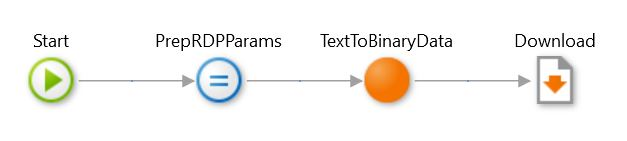
\includegraphics[width=\linewidth]{rdp.JPG}
        \caption{Client actie om een RDP file te genereren.}
    \end{subfigure}
    \begin{subfigure}[b]{0.4\linewidth}
        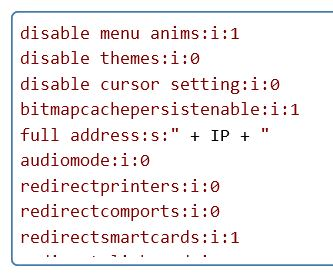
\includegraphics[width=\linewidth]{rdp-sjab.JPG}
        \caption{Deel van de RDP configuratie waar het IP-adres en gebruikersnaam ingevuld worden.}
    \end{subfigure}
    %\caption{Overzicht van de filtering voorbereidingen.}
    \label{fig:rdp-actie}
\end{figure}

\textit{Ping}

De basis van het probleem bij het uitwerken van RDP geldt ook hier. Toestellen zijn enkel benaderbaar in het lokale netwerk, de ping moet dus uitgevoerd kunnen worden aan de client kant. Outsystems maakt uitvoeren van client side javascript mogelijk maar er werd geen oplossing gevonden om Ping op deze manier te laten slagen.\\
Plan B is om een extensie te maken. In de persoonlijke omgeving moet dit in .NET en hier is het onder andere mogelijk om de Pinger\footnote{ASP.NET C\# Helper Class to execute a ICMPv4 PING to any remote host using hostname or IP Address - \url{https://www.ryadel.com/en/asp-net-c-sharp-icmpv4-ping-remote-host-hostname-ip-address/}} klasse te implementeren. Een grote opmerking hierbij is dat de app on-premises gehost moet worden om dit echt te laten werken.

Stappen om de extensie aan te maken:
\begin{enumerate}
    \item Een nieuwe extensie aanmaken in Integration Studio.
    \item De actie 'PingHost' declareren. Er zijn twee parameters nodig:\\
    $\rightarrow$ ipaddress (Text)\\
    $\leftarrow$ pingable (Boolean)
    \item Visual Studio openen met de 'Edit Source Code .NET' knop.
    \item Een methode schrijven die de Pinger klasse implementeert (Zie Listing~\ref{lst:pinger-meth}). 
    \item Net als in de Service Studio One Click-Publish gebruiken om de extensie op te slaan en beschikbaar te maken.
    \item De extensie als dependency toevoegen aan de POC maakt de PingHost actie bruikbaar.
\end{enumerate}

Deze eenvoudige methode maakt een instantie van de Pinger klasse, stuurt de ping naar het IP-adres van de invoerparameter en evalueert het resultaat op succes om dit als boolean uitvoer terug te sturen. 
\begin{lstlisting}[style=CSharpStyle,label={lst:pinger-meth},caption={Pinger implementatie},captionpos=b]
public void MssPingHost(string ssipaddress, out bool sspingable) {
    sspingable = false;
    using (Ping pinger = new Ping())
    {
        try
        {
            PingReply reply = pinger.Send(ssipaddress);
            sspingable = reply.Status == IPStatus.Success;
        }
        catch (PingException e)
        {
        sspingable = false;
        }
    }
}
\end{lstlisting}

\subsubsection{Mobiel bruikbaar zijn}

Het gekozen soort app is reactive om zowel op desktop als mobiele layout bruikbaar te zijn maar er werd niet verwacht dat er bij deze keuze (tussen Traditional Web, Reactive en Mobile) functionaliteit verloren zou gaan. Dit was wel het geval:
\begin{itemize}
    \item \textbf{Automatisatie:} Het maken van een Timer die mail verstuurt is enkel mogelijk in een Tradional Web App, er was een workaround nodig (Zie Subsectie~\ref{subsec:os-automatisatie}).
    \item \textbf{Barcode Scanning:} Een Mobile App is nodig om de Barcode Scanner te kunnen gebruiken (Zie Subsectie~\ref{subsec:os-barcode}).
\end{itemize}

\begin{figure}[h!]
    \centering
    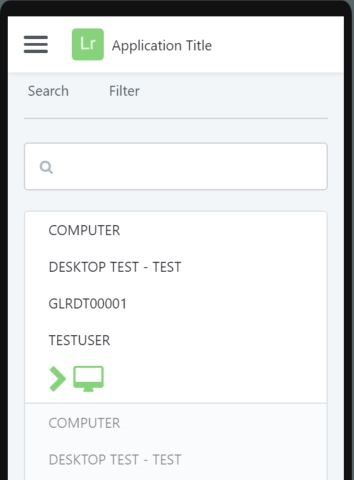
\includegraphics[width=0.4\linewidth]{os-hoofd-mobile-cut.JPG}
    \caption{Voorbeeld van de POC met een mobiele layout.}
    \label{fig:os-hoofd-mobile}
\end{figure}

\subsubsection{Future proof zijn}

Een indicator is de marktpositie. Zowel Gartner als Forrester bestempelen Outsystems als leider (Zie Tabel~\ref{table:leiders}). Dit spreekt positief over de bestaanszekerheid.\\
Ook hun traject over de jaren geeft vertrouwen.
Outsystems is opgericht in 2005 en sinds dan is het product en de licentiëring ervan consistent gebleven.\\
Hierbovenop komt dat er steeds vernieuwingen worden geïntroduceerd\footnote{Product Releases and Updates - \url{https://www.outsystems.com/whats-new/}}.
% TODO: volwaardige bron vinden?

\subsubsection{Performant zijn}

Een app in de cloud is meestal niet zo snel als een lokale applicatie. Zeker ophalen van data over het internet heeft een invloed op performantie.\\
Hoe weegt deze POC dan op tegen de PowerApps POC?\\
In Subsectie~\ref{subsec:os-prijs} wordt een beeld gevormd van de beperkingen. Vooral de punten over gedeelde resources en 'in slaap gaan' van de omgeving zijn relevant ten opzichte van performantie. PowerApps kent deze beperkingen niet. Dit is natuurlijk te verwachten als een gratis plan (Outsystems) vergeleken wordt met een betalend plan (PowerApps).\\
Er kan dus besloten worden dat PowerApps consistentere performantie zal bieden.

\subsubsection{Security}

% TODO: gdpr bron
De POC is toegankelijk met geldige Outsystems credentials. Alternatieve user management (bijvoorbeeld Azure Active Directory) is mogelijk maar niet in de gratis versie en in geval van Azure moet de App on premises gehost worden.

\subsection{Should have}

\subsubsection{Gerichte/basis taken kunnen automatiseren}
\label{subsec:os-automatisatie}

Net als bij de PowerApps POC bestaat de case uit het wekelijks genereren en uitsturen van een rapport met toestellen die langer dan een maand 'te schrappen' staan.\\
Voor herhalende taken zijn Timers in te stellen. Het probleem is dat het in Traditional Web apps mogelijk is om mails te versturen in acties maar dat deze functionaliteit voor Reactive Web apps (nog) niet ondersteund is. Als workaround is gekozen om een aparte Traditional Web app te maken die het uitvoeren van deze stappen overneemt.

Voorbereidend moet de omgeving in Service Center geconfigureerd worden om e-mail te kunnen versturen. Dit gebeurt in Administration > Email. Meest notabel zijn de te gebruiken SMTP Server en standaard afzenderadres. Het is ook mogelijk om voor testscenario's al de mails te redirecten naar een testlijst.

Eens een nieuwe Traditional Web app is aangemaakt in de Service Studio volstaat het om:
\begin{enumerate}
    \item Wat logica betreft: één server actie declareren met één 'Send Email' stap.
    \item De mail body configureren: belangrijkst is een Table dat het overzicht van de devices zal bevatten.
    \item De asset databank uit de hoofd POC module als dependency declareren en toevoegen aan de Table. Dit maakt er automatisch een aggregate voor aan in een nieuwe Preparation stap. Elke keer de mail opgesteld wordt zal deze Preparation stap eerst uitgevoerd worden.
    \item In deze aggregate wordt een filter ingesteld om de juiste toestellen terug te geven.
\begin{lstlisting}
AddMonths(testdata.SCHRAPSINDS,1) <= CurrDateTime() and testdata.KLEUR = "BLAUW"
\end{lstlisting} 
    \item Een timer instellen om de actie uit stap één op een tijdschema uit te voeren (Zie Figuur~\ref{fig:mail-timer})
\end{enumerate}

\begin{figure}[h!]
    \centering
    \begin{subfigure}[b]{0.5\linewidth}
        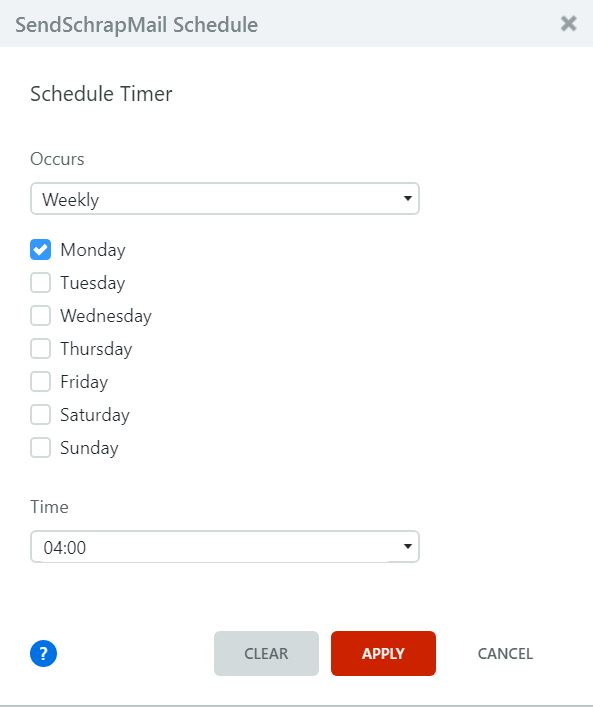
\includegraphics[width=\linewidth]{timer-schedule.JPG}
        \caption{Bepalen van het tijdschema voor de Mail Timer.}
    \end{subfigure}
    \begin{subfigure}[b]{0.45\linewidth}
        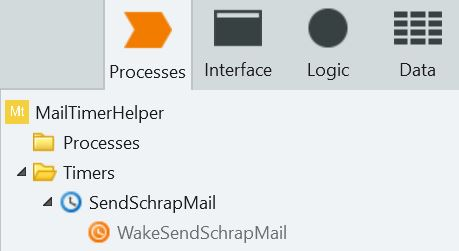
\includegraphics[width=\linewidth]{mailtimer.JPG}
        \caption{Mail Timer context overzicht.}
    \end{subfigure}
    \begin{subfigure}[b]{0.6\linewidth}
        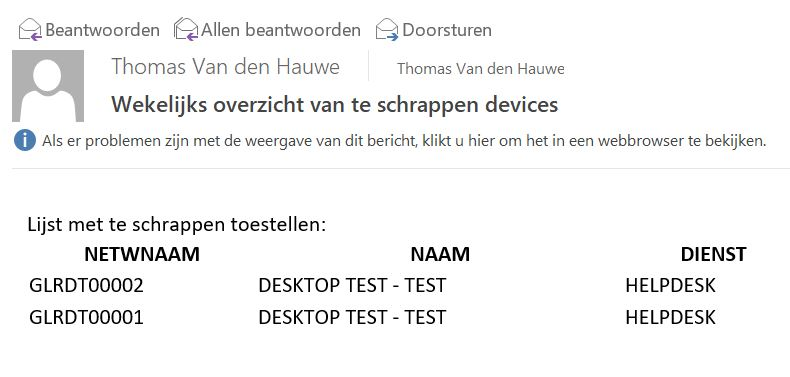
\includegraphics[width=\linewidth]{res-mail-os.JPG}
        \caption{Voorbeeld van het resultaat.}
    \end{subfigure}
    \caption{Overzicht van de configuratie en het resultaat van de Mail Timer.}
    \label{fig:mail-timer}
\end{figure}

\subsubsection{Bruikbaar zijn buiten domein}

De POC en databank zijn cloud gehost. Enkel internettoegang en Outsystems credentials zijn nodig om de POC te kunnen gebruiken.

\subsubsection{SharePoint requirements}

Requirements die met SharePoint te maken hebben zijn:
\begin{itemize}
    \item Nieuwe types toestellen opnemen.
    \item Randapparatuur opnemen.
    \item Revisie van elk dataveld per toesteltype.
    \item Data opslaan in SharePoint (cloud).
\end{itemize}
Dit wordt besproken in Sectie~\ref{sec:sharepoint}.

\textit{Onderstaande aanpak werd onderzocht maar na afloop niet toegepast. Voor het huidige scenario voldoet de standaard voorziene SQL instantie en zijn er geen merkbare voordelen die de extra complexiteit verantwoorden.}

Er is geen connector zoals in PowerApps dat rechtstreekse toegang geeft tot de SharePoint data. De verbinding zal met andere woorden via de beschikbare REST api's moeten verlopen. SharePoint heeft zijn eigen '\_api' toegang, alternatief is er ook de nieuwere Microsoft Graph. Omdat in de PowerApps POC Graph reeds gebruikt werd (Subsectie~\ref{subsec:ms-graph}) wordt er hier opnieuw voor gekozen. Iets dat daar aan bod kwam was het verschil tussen delegated en application permissions. Ook hier wordt uitgegaan van delegated permissions gezien dit de veiligere optie is (Windows login nodig).

Alvorens er data opgevraagd kan worden moet het autorisatieproces (hier OAuth V2) doorlopen worden (Figuur~\ref{fig:auth-proces}).

\begin{figure}[h!]
    \centering
    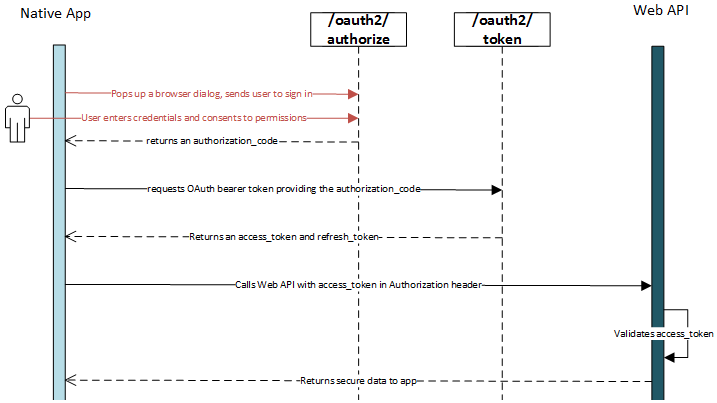
\includegraphics[width=\linewidth]{auth-proces.png}
    \caption{Weergave van het autorisatieproces. \autocite{MSLCT2019}}
    \label{fig:auth-proces}
\end{figure}

De implementatie ervan in Outsystems gaat als volgt:
\begin{enumerate}
    \item Azure
    \begin{enumerate}
        \item App registratie.
        \item Client secret aanmaken.
        \item Scope definiëren. Voor SharePoint is dit: \lstinline|Sites.Manage.All Sites.Read.All SitesReadWrite.All|
        \item Redirect URL naar de Outsystems app instellen. Structuur is \lstinline|https://<outsystems omgeving>/<app naam>/<afhandeling pagina>| 
    \end{enumerate}
    \item Autorisatie request doen(\lstinline|\authorize| eindpunt). Komt overeen met inloggen in Windows account en goedkeuren van de scope.\\
    $\leftarrow$ Autorisatiecode wordt teruggegeven.
    \item Token aanvragen met de autorisatiecode (\lstinline|\token| eindpunt)\\
    $\leftarrow$ Token wordt teruggegeven.
\end{enumerate}
Dit token moet aanwezig zijn in elke request naar de SharePoint data via Microsoft Graph.

Het is echter mogelijk een deel van deze stappen door te geven naar een Forge component (zoals Microsoft Login Connector Reactive \autocite{MSLCT2019}). De implementatie daarvan is een pak eenvoudiger: in de standaard login actie van de POC wordt de methode uit de extensie geplaatst die het autorisatieproces start 'GetOAuth2AuthenticationURL'. Praktisch gezien wordt na de Outsystems login nu ook de Microsoft login uitgevoerd. Na afloop is het token beschikbaar om te gebruiken in REST operaties. Alleen de voorbereiding in Azure moet nog steeds gedaan worden.

\subsubsection{Leercurve moet degelijk zijn}

\textit{(Dit deel is gebaseerd op persoonlijke ervaringen van de auteur)}

De algemene leercurve van Outsystems ligt hoger dan bij PowerApps, dit is logisch omdat het om een andere doelgroep gaat.\\
Als er specifieker gekeken wordt naar de oorzaken van moeilijkheid tussen beide platformen:
\begin{itemize}
    \item \textbf{Outystems:} Gebruik van data en datatypen kan in sommige scenario's overweldigend zijn voor een beginner.
    \item \textbf{PowerApps:} Gebruik van formules en vooral sommige technieken die er mee gebruikt moeten worden.
\end{itemize}

Over hulpmateriaal:\\
De documentatie is goed en de community is actief. De instructievideo's zijn ok. Deze zijn van Outsystems zelf maar soms verouderd.\\
Community apps uit de Forge zijn ook handig. Componenten kunnen ingekeken worden specifiek om technieken aan te leren. Veel forge apps zijn als demo bedoeld of hebben een companion demo app.

\subsection{Nice to have}

\subsubsection{Samenwerken met SCCM en/of synchroniseren met en data uit de SQL databank kunnen gebruiken}

% todo: powerapps methode aan te passen om ook hier te gebruiken?
Dit valt buiten de scope van het onderzoek.

\subsubsection{Diverse GUI verbeteringen/robuust GUI ontwerp ondersteunen}

Om de GUI te bouwen wordt het UI framework genaamd Silk UI\footnote{\url{https://silkui.outsystems.com/}} gebruikt. Er is een grote focus op Drag-en-drop.

Een overzicht van Silk UI componenten, die telkens meer controle over detail geven:

\textit{Screen templates $\rightarrow$ thema editor $\rightarrow$ UI patronen/controls voor gangbare use cases $\rightarrow$ Style properties $\rightarrow$ CSS editor}

Afhankelijk van hoeveel tijd men wil spenderen is elk aspect van de UI met andere woorden aan te passen.

De gemaakte POC is reactive. Een samenvatting van de ervaringen bij het bouwen van de UI is dat er veel controle is over details maar dat drag-en-drop warrig kan worden als er veel containers/componenten op het scherm zijn.

\subsubsection{Barcodes kunnen scannen}
\label{subsec:os-barcode}

Dit is mogelijk via het officiële Forge Component van Outsystems\footnote{\url{https://www.outsystems.com/forge/component-overview/1403/barcode-plugin}}.\\
Na het importeren van de barcode scanner als dependency is het gebruik ervan analoog met de variant in PowerApps.
\begin{enumerate}
    \item Een knop toevoegen bij de Text Input horend bij de kolom waar de later ingescande waarde ingevuld zal worden. Dit is in de Form widget op het detailscherm.
    \item Een Client actie declareren op het On Click event die 'ScanBarCode' oproept en de 'ScanResult' parameter aan een variabele koppelt.
    \item Deze variabele instellen als inhoud van de doel Text Input (MAC of SERIAL).
\end{enumerate}

Bij de uitwerking werden snel problemen vastgesteld. Omdat de POC een Reactive Web app is zijn de nodige Apache Cordova componenten niet beschikbaar. Dit is beperkt tot een Mobile app en de POC zou als dusdanig moeten herschreven worden om de Barcode Scanner effectief te kunnen gebruiken.

\subsubsection{AI functionaliteit}

Geen enkele van de opgestelde requirements heeft AI nodig. Dit werd niet verder onderzocht.

% TODO: extra uitleg tov wat in requirementsanalyse staat.